\section{Implementation}																	
\label{sec:Implementation}

\subsection{Overview} 
This section goes into details on the implementation of the Course Creator and Virtual Reality Orienteering programs. Key examples and general explanations are presented, to help the reader understand the code without rehashing the entire project. 

\subsection{Course Creator}
The Course Creator's primary responsibilities is creating courses and viewing results of those courses. Courses are comprised of locations, questions, and answers; each course has many locations, each location has many questions, and each question has many answers. 

\subsubsection{Authorization}
The Course Creator uses ASP.NET Core Identity to secure the application. This tool makes creating the registration and login pages simple, and has built-in security for securely storing passwords and other personal user data. ASP.NET Core Identity also makes use of user roles to ensure the user is authorized to do certain actions. The verified user role is an example of this in the project. Using a filter on the protected controllers is simple with Identity.
\begin{lstlisting}[caption=Securing Controllers using Filter on User Role, label=lst:FilterUserRole]
using Microsoft.AspNetCore.Authorization;

[Authorize(Roles = "Verified")]
public class HomeController : Controller
{
	...
}
\end{lstlisting} 
\subsubsection{Courses}
The course is the high level object with which the locations, questions, and answers become associated with. A course can be added, updated, or deleted. The \lstinline{CoursesController} handles all of these actions. Each of these actions has a corresponding View Razor page. The basic course model looks like the following:
\begin{lstlisting}[caption=Course Model, label=lst:CourseModel]
public class Course
{
	public int CourseId { get; set; }
	
	[DisplayName("Name")]
	public string Name { get; set; }

}
\end{lstlisting}
 
 The create and edit pages are similar to the other pages for the locations, questions, and answers, so this section will not go in depth on them, but instead elaborate further on the details and delete pages. The details page displays not only the course model information, but also all information relating to the course. To make the related course information modularize and reusable, the developer made use of ``View Components". View Components render a chunk of HTML output within another markup's file. This breaks up large markup files into smaller parts, reduces duplication of markup content, and provides an opportunity to use logic to control the rendered HTML. Each of the dependent classes on a course has a corresponding View Component which lists the data relating to the course. This can be seen in Listing \ref{lst:CourseDetails} of the course details page on line 30:
 \begin{lstlisting}[style=htmlcssjs, caption=Course Details Razor Page, label=lst:CourseDetails]
 @model ImmersiveQuiz.Models.Course
 
 @{
 ViewData["Title"] = "Details";
 }
 
 <h1>Details</h1>
 
 <div>
	 <h4>Course</h4>
	 <hr />
	 <dl class="row">
		 <dt class="col-sm-2">
			 @Html.DisplayNameFor(model => model.Name)
		 </dt>
		 <dd class="col-sm-10">
			 @Html.DisplayFor(model => model.Name)
		 </dd>
	 </dl>
 </div>
 <div class="mb-4">
	 <a class="badge large-badge bg-secondary text-light" asp-action="Index">Back to List</a> |
	 <a class="badge large-badge bg-success text-light" asp-controller="Scores" asp-action="Index" asp-route-id="@Model.CourseId">Scores</a>
 </div>
 <div>
	 <a class="badge large-badge bg-success text-light" asp-action="Create" asp-controller="Locations" asp-route-id="@Model.CourseId">Add Location</a> |
	 <a class="badge large-badge bg-primary text-light" asp-action="Edit" asp-route-id="@Model.CourseId">Edit</a>
	 <a class="badge large-badge bg-danger text-light" asp-action="Delete" asp-route-id="@Model.CourseId">Delete</a> 
 </div>
 @await Component.InvokeAsync("LocationList", new { CourseId = Model.CourseId.ToString(), search = "" })
 \end{lstlisting}
 
 Another area of interest for the Courses is the delete action. A course could be deleted independent of the dependencies which destroys the concept of Referential Integrity, which is \qquote{a database concept that is used to build and maintain logical relationships between tables to avoid logical corruption of data.}{refInteg} When data is deleted independently, the dependencies now have a reference to data that no longer exists. This corrupts the reliability of the data. To counter this the developer made use of cascading deletes. That is to say, when a course is deleted, the delete cascades onto the locations, questions, and answers dependent on that course. The cascading delete can be seen in Listing \ref{lst:CourseDelete} using LINQ, Entity Framework Core, and Dependency Injection.
 \begin{lstlisting}[caption=Course Cascade Delete, label=lst:CourseDelete]
 [HttpPost, ActionName("Delete")]
 [ValidateAntiForgeryToken]
 public async Task<IActionResult> DeleteConfirmed(int id)
 {
	 var course = await _courseContext.Course.FindAsync(id);
	 
	 var locations = _locationContext.Location.Where(l => l.CourseId == course.CourseId);
	 
	 foreach (var location in locations)
	 {
		 var questionsToLocations = _questionContext.Question.Where(q => q.LocationId == location.LocationId);
		 foreach (var question in questionsToLocations)
		 {
			 var answersToQuestion = _answerContext.Answer.Where(ans => ans.QuestionId == question.QuestionId);
			 _answerContext.Answer.RemoveRange(answersToQuestion);
			 
			 _questionContext.Remove(question);
		 }
		 _locationContext.Location.Remove(location);
	 }
	 
	 _courseContext.Course.Remove(course);
	 
	 await _answerContext.SaveChangesAsync();
	 await _questionContext.SaveChangesAsync();
	 await _locationContext.SaveChangesAsync();
	 await _courseContext.SaveChangesAsync();
	 
	 return RedirectToAction(nameof(Index));
 }
 \end{lstlisting}
 
\subsubsection{Locations}
The Location is the container for the questions and answers. The Location is also responsible for the management of the 360 photos. While it is possible to store images and files directly into the database using BLOBS, this is inefficient in storage and retrieval. Instead the developer made use of File System storage. Thus, the location's database record instead contains a reference to where the image lives, rather than the image itself. A location can be added, updated, or deleted. The \lstinline{LocationsController} handles all of these actions. Each of these actions has a corresponding View Razor page. The Location model is shown in Listing \ref{lst:LocationModel}.
\begin{lstlisting}[caption=Location Model, label=lst:LocationModel]
public class Location
{
	public int LocationId { get; set; }
	
	public string Name { get; set; }
	
	public Guid ImageGuid { get; set; }
	
	public string ImageExtension { get; set; }
	
	public string ImagePath {
		get
		{
			return $"/images/{ImageGuid}{ImageExtension}";
		}
	}

	public int CourseId { get; set; }
	
	[NotMapped]
	public Course Course { get; set; }
}
\end{lstlisting}

The Location keeps track of the \lstinline{ImageGuid} and \lstinline{ImageExtenstion} to create the \lstinline{ImagePath}. Each uploaded image is given a globally unique identifier (GUID) which \qquote{is a 128-bit number created by the Windows operating system or another Windows application to uniquely identify specific components, hardware, software, files, user accounts, database entries and other items.}{guidDef}. Assigning each image with a GUID guarantees unique image file names when storing in the File System storage and discourages malicious users from scrapping the File System with predictive names. The process for uploading a new image can be seen in Listing \ref{lst:ImageUpload}.
\begin{lstlisting}[caption=Uploading an Image, label=lst:ImageUpload]
private Guid UploadImage(IFormFile image)
{
	Guid imageGuid = Guid.NewGuid();
	string filePath = Path.Combine(Path.Combine(_webHostEnvironment.WebRootPath, "images"), imageGuid.ToString()) + Path.GetExtension(image.FileName);
	
	using var fileStream = new FileStream(filePath, FileMode.Create);
	image.CopyTo(fileStream);
	
	return imageGuid;
}
\end{lstlisting} 

\subsubsection{Questions}
The Question is the container for answers and contains the content for question being asked. A question can be added, updated, or deleted. The \lstinline{QuestionsController} handles all of these actions. Each of these actions has a corresponding View Razor page. The Question model is shown in Listing \ref{lst:QuestionModel}.
\begin{lstlisting}[caption=Question Model, label=lst:QuestionModel]
public class Question
{
	public int QuestionId { get; set; }
	
	[DisplayName("Question")]
	public string Content { get; set; }
	
	public int LocationId { get; set; }
	
	[NotMapped]
	public Location Location { get; set; }
	
	[NotMapped]
	public List<Answer> Answers { get; set; }
}
\end{lstlisting}

\subsubsection{Answers}
The Answer is the lowest-level object for the Course Creator, containing nothing but the answer content and a boolean for a correct answer.  A answer can be added, updated, or deleted. The \lstinline{AnswersController} handles all of these actions. Each of these actions has a corresponding View Razor page. The Answer model is shown in Listing \ref{lst:AnswerModel}.
\begin{lstlisting}[caption=Answer Model, label=lst:AnswerModel]
public class Answer
{
	public int AnswerId { get; set; }
	
	[DisplayName("Answer")]
	public string Content { get; set; }
	
	public int QuestionId { get; set; }
	
	[DisplayName("Correct Answer")]
	public bool IsCorrect { get; set; }
	
	[NotMapped]
	public Question Question { get; set; }
}
\end{lstlisting}

\subsubsection{Course Results}
The course results is handled by the Score class which contains the student ID, Time Score, and Point Score. The Total Score is calculated by read only property which adds the time score and point score together.  A score can be added, updated, or deleted to give a verified user full control over the scores. The scores will typically come from the Virtual Reality Orienteering program in a POST request. The \lstinline{ScoresController} handles all of these actions. Each of these actions has a corresponding View Razor page. The Score model is shown in Listing \ref{lst:ScoreModel}.
\begin{lstlisting}[caption=Score Model, label=lst:ScoreModel]
public class Score
{
	public int ScoreId { get; set; }
	
	[DisplayName("Student ID")]
	public string StudentId { get; set; }
	
	public int CourseId { get; set; }
	
	[DisplayName("Time Score")]
	public decimal TimeScore { get; set; }
	
	[DisplayName("Point Score")]
	public decimal PointScore { get; set; }
	
	public decimal TotalScore { 
		get 
		{
			return TimeScore + PointScore;
		}
	}
}
\end{lstlisting}
\subsubsection{Web API}
The Web API is a RESTful API which controls all of the allowed external endpoints. This Web API is how the Virtual Reality Orienteering program is able to communicate with the Course Creator. Courses are loaded and scores submitted via requests to this Web API. The Web API is secured using a filter with Basic Authentication and a HTTPS connection. Using a tool called Swagger the request documentation is auto generated, providing an easy visualization of the endpoints, schema, and resources available for the Web API. The endpoints can be seen in Figure \ref{fig:WebApiEndpoints}.
\begin{figure}[htb]
	\centering
	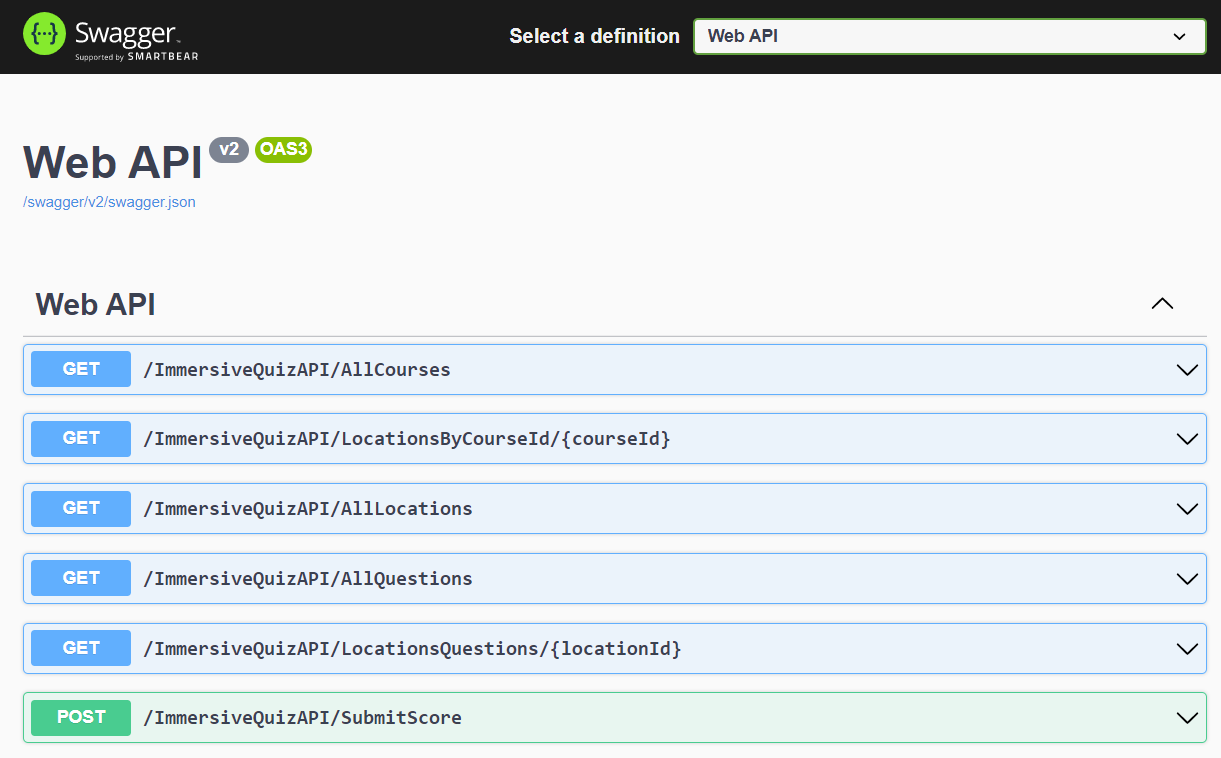
\includegraphics[width=.9\textwidth]{Implementation/assets/web-api-endpoints.png}
	\caption[Web API Endpoints]{\label{fig:WebApiEndpoints}Web API Endpoints}
\end{figure}

Swagger also auto generates the class schema for the request body's that the endpoints use. The Web API sends only the needed model information and nothing more. Thus, business objects of each of the main components of the Course Creator are used to simplify the requests. These objects can been seen in Figure \ref{fig:WebApiSchema}.
\begin{figure}[htb]
	\centering
	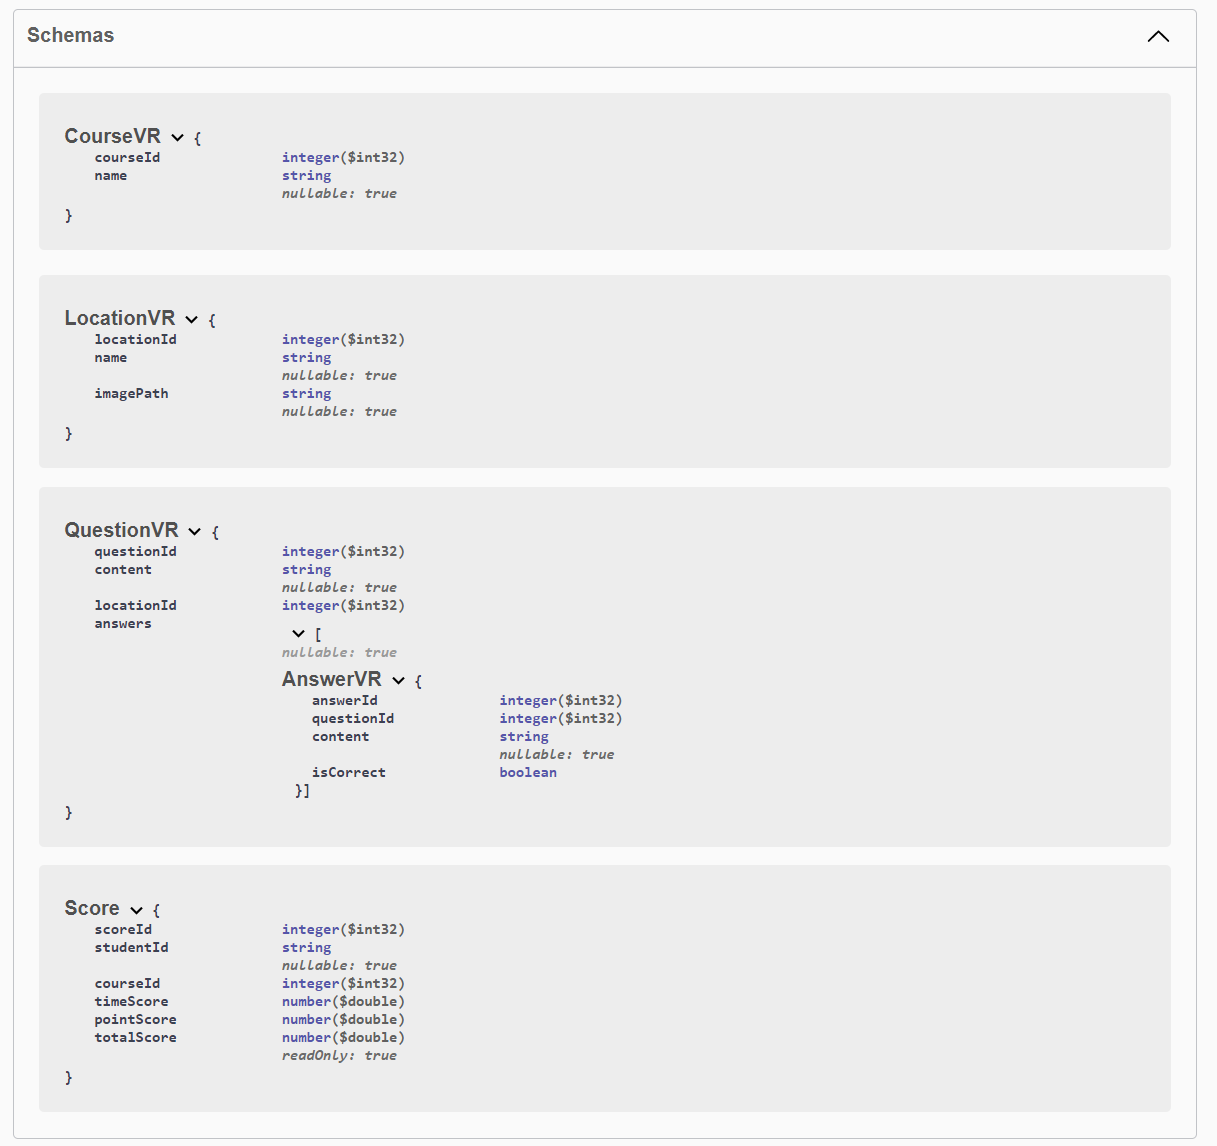
\includegraphics[width=.9\textwidth]{Implementation/assets/web-api-schema.png}
	\caption[Web API Schema]{\label{fig:WebApiSchema}Web API Schema}
\end{figure}

\subsection{Virtual Reality Orienteering}
The Virtual Reality Orienteering primary responsibilities are to display the course and to keep track and submit the results. The Virtual Reality Orienteering program must have authorized communication with the Course Creator program.

\subsubsection{Authorization}
The Virtual Reality Orienteering makes use of Basic Authentication to securely make requests to the Web API in the Course Creator. To access the Virtual Reality Orienteering program the student must be physically present on a computer with
a headset, the Course Creator program, and the Virtual Orienteering program. The instructor will proctor the student to ensure the student ID and chosen course is correctly entered. 

\subsubsection{Displaying a Course}
The Virtual Reality Orienteering makes requests to the Web API to get course data. Once a student has entered their student ID, they must select a course. The Virtual Reality Orienteering program calls the endpoint \lstinline{GET /ImmersiveQuizAPI/AllCourses} to display this list of courses. Once a course is selected, a call is made to the \lstinline{GET /ImmersiveQuizAPI/LocationsByCourseId/}\{\lstinline{courseId}\} to get all locations for the course. As each location is loaded, another call is made to the \lstinline{GET /ImmersiveQuizAPI/LocationsQuestions/}\{\lstinline{locationId}\} to load the questions and corresponding answers for each location. 

\subsubsection{Tracking and Submitting Score Results}
In the spirit of orienteering, each location is timed to completion and is added to the total score. A Timer class is associated with the main controller, \lstinline{VRInputModule}, and provides the functionality for keeping track of the time and returning the time as a score. Listing \ref{lst:timer} shows a snippet of the Timer class and the code for the \lstinline{Update()} which is updated every frame.
\begin{lstlisting}[caption=Timer Update Snippet,label=lst:timer]
using UnityEngine;
using UnityEngine.UI;

public class Timer : MonoBehaviour
{
	public static float startTime = 100;
	public float timeRemaining = startTime;
	public bool timerIsRunning = false;
	
	...
	
	void Update()
	{
		if (timerIsRunning)
		{
			if (timeRemaining > 0)
			{
				timeRemaining -= Time.deltaTime;
			}
			else
			{
				// Time ran out!
				timeRemaining = 0;
				timerIsRunning = false;
			}
		}
	}

	...

}
\end{lstlisting} 

Throughout the progress of the course, the point score and time score are kept track of in aggregate. When all locations have been completed the UI displays a game over message with the point score, time score, and total score. The Virtual Reality Orienteering program then makes a call to the Web API to \lstinline{POST /ImmersiveQuizAPI/SumbitScore} with the JSON body of \{\lstinline{studentId: "string", courseId : int, timeScore: float, pointScore: float}\}. The \lstinline{SubmitScore()} method making the call to the Web API is shown in Listing \ref{lst:SubmitScore}.
\begin{lstlisting}[caption=Sumbit Score, label=lst:SubmitScore]
private IEnumerator SubmitScore(string studentId, float timeScore, float pointScore)
{
	var json = JsonConvert.SerializeObject(new { studentId, CourseLibrary.Courses[currentCourse].CourseId, timeScore, pointScore });
	var request = new UnityWebRequest($"{WebApi}/ImmersiveQuizAPI/SubmitScore", "POST")
	{
	 uploadHandler = new UploadHandlerRaw(Encoding.UTF8.GetBytes(json)),
	 downloadHandler = new DownloadHandlerBuffer()
	};
	
	request.SetRequestHeader("Content-Type", "application/json");
	request.SetAuthHeader();
	
	yield return request.SendWebRequest();
}
\end{lstlisting}

